\documentclass[11pt, oneside]{article}   	% use "amsart" instead of "article" for AMSLaTeX format
\usepackage{geometry}                		% See geometry.pdf to learn the layout options. There are lots.
\geometry{letterpaper}                   		% ... or a4paper or a5paper or ... 
%\geometry{landscape}                		% Activate for for rotated page geometry
%\usepackage[parfill]{parskip}    		% Activate to begin paragraphs with an empty line rather than an indent
\usepackage{graphicx}				% Use pdf, png, jpg, or eps� with pdflatex; use eps in DVI mode
								% TeX will automatically convert eps --> pdf in pdflatex		
\usepackage{amssymb}
\usepackage{amsmath}
\usepackage{parskip}
\usepackage{color}

\title{Shankar Exponential}
%\author{The Author}
%\section{}
% \subsection*{R code}
\date{}							% Activate to display a given date or no date

\graphicspath{{/Users/telliott_admin/Dropbox/Tex/png/}}

% \begin{center} 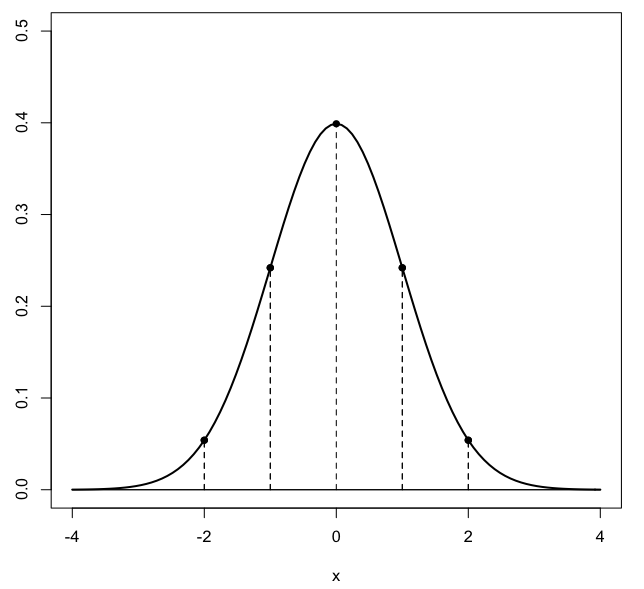
\includegraphics [scale=0.4] {gauss3.png} \end{center}

\begin{document}
\maketitle
\Large
\noindent
\begin{quote}To this end, let us now ask what $a^x$ means for any $x$.  Note that $x$ is now the exponent, not the base.  This is because we want to vary the exponent continually over all real values, and wish to denote this variable by $x$.  To define $a^x$, we compute its derivative with respect to $x$.  You may wonder how we can compute the derivative of something before having defined it!  Watch!\end{quote}
\[ \Delta a^x = a^{(x+\Delta x)} - a^x \]
\[ = a^x(a^{\Delta x} - 1) \]
We are trying to write an expression for $a^{\Delta x}$, near $x=0$.  It will be very close to $1$ since $a^0 = 1$.  Using the method of the Taylor series we write
\[ a^{\Delta x} \approx 1 + \ln(a) \Delta x + \dots \]
Here $\ln$ is a new function (which will turn out to have all the properties of, and hence be equal to, the natural logarithm).  At the moment, all we know is that the first order correction term is some function of $a$.  So
\[ \Delta a^x = a^x(1 + \ln(a) \Delta x + \dots - 1) \]
The two $1$'s cancel, and the dots are higher powers of $\Delta x$ which will go away when we take the limit.
\[ \frac{d}{dx} a^x = a^x \ln(a) \]
Shankar has a discussion leading to the conclusion that for some value $e > 1$, it will be true that $\ln(e) = 1$ so then
\[ \frac{d}{dx} e^x = e^x \]
Now we can find the value of $e^x$ near $x=0$ as
\[ e^x = \sum_{n=0}^{n=\infty} \ \frac{f^n(0)}{n!} x^n \]
In particular, all the derivatives are just $e^x = 1$ at $0$ so
\[ e^x = \sum_{n=0}^{n=\infty} \ \frac{x^n}{n!} \]
\[ = \frac{x^0}{0!} + \frac{x}{1!} + \frac{x^2}{2!} + \frac{x^3}{3!} \dots \]
and if $x=1$ we have that
\[ e^1 = e = 1 + 1 + \frac{1}{2!} + \frac{1}{3!} \dots \]
Don't be concerned by the fact that we are evaluating $e^x$ and $x=1$ using the derivatives evaluated at $x=0$.  The series is exact for any $x$ \emph{as long as we take enough terms}.

The first three terms are equal to $2.5$.  The next three terms are $1/6 = 0.16 \dots$, $1/24 = 0.0416 \dots$, and $0.0083 \dots$ which sum to $0.216 \dots$, and added to $2.5$ come fairly close to the true value of $e=2.718281828 \dots$.  The sum converges quickly because the factorial grows so fast in the denominator.

\end{document}  